\documentclass[conference]{IEEEtran}
\IEEEoverridecommandlockouts

\usepackage{amsmath,amssymb,amsfonts}
\usepackage{algorithmic}
\usepackage{algorithm}
\usepackage{graphicx}
\usepackage{textcomp}
\usepackage{xcolor}
\usepackage{booktabs}
\usepackage{cite}
\usepackage{tikz}
\usepackage{pgfplots}
\pgfplotsset{compat=1.18}
\usetikzlibrary{arrows.meta,positioning,shapes.geometric,fit,backgrounds}

\begin{document}

\title{FitScore AI: A Real-Time Biomechanical Quality Scoring and Injury Prevention Framework Using Spatial-Temporal Pose Kinematics and Hybrid Deep Learning}

\author{
\IEEEauthorblockN{Preethi R.\IEEEauthorrefmark{1}, Ramyashri Ravikumar\IEEEauthorrefmark{1}, Vaishnavi G.~N.\IEEEauthorrefmark{1}, Vaishnavi S.\IEEEauthorrefmark{1}, and Yashaswini C.~D.\IEEEauthorrefmark{2}}
\IEEEauthorblockA{Department of Computer Science and Engineering (Data Science)\\
AMC Engineering College, Visvesvaraya Technological University, Bengaluru, Karnataka, India\\
Email: \IEEEauthorrefmark{1}\{1am23cd078, 1am23cd086, 1am23cd115, 1am23cd116\}@amcec.edu.in, \IEEEauthorrefmark{2}yashaswinicd@amcec.edu.in}
}

\maketitle

\begin{abstract}
Quantitative assessment of physical exercise form is vital for both athletic conditioning and tele-rehabilitation. However, existing remote solutions typically offer either binary feedback (e.g., correct versus incorrect repetitions) or rely on specialized, cost-prohibitive motion-capture equipment. In this work, we propose FitScore AI, an accessible browser-based framework that computes continuous biomechanical quality scores in real time using a standard monocular webcam. The system extracts 33 three-dimensional anatomical landmarks via MediaPipe BlazePose and applies a torso-centered, scale-invariant spatial normalization. Movement classification across 19 rehabilitation and resistance exercise classes is carried out using a hybrid Convolutional Neural Network and Long Short-Term Memory (CNN-LSTM) architecture, augmented with a Finite State Machine (FSM) repetition gate. We formulate a composite continuous metric, the FitScore ($0$--$100$), derived from four biomechanical pillars: Range of Motion (ROM), movement symmetry, cadence tempo, and joint trajectory stability. Concurrently, an analytical injury risk stratification engine identifies unsafe movement compensations, such as dynamic knee valgus and lumbar spinal flexion. Across extensive ablation experiments, our deployed architecture achieves 93.6\% sequence classification accuracy, 0.929 precision, 0.924 recall, and an F1-score of 0.926, while maintaining an end-to-end processing latency below 65\,ms.
\end{abstract}

\begin{IEEEkeywords}
Exercise quality scoring, pose estimation, CNN-LSTM, biomechanical kinematics, injury risk detection, tele-rehabilitation, MediaPipe BlazePose.
\end{IEEEkeywords}

\section{Introduction}

Musculoskeletal rehabilitation and resistance exercise regimens demand rigorous execution to maximize therapeutic efficacy and prevent acute joint injury \cite{hewett2005biomechanical}. While certified physiotherapists and athletic trainers provide personalized supervision in clinical environments, high costs and geographic constraints limit access for home-based users and tele-rehabilitation patients \cite{woo2024exercise}. 

Optical marker-based motion capture (MoCap) systems, such as Vicon, serve as the clinical gold standard for joint angle quantification \cite{vanderkruk2018present}. Nevertheless, their requirement for multi-camera laboratory installations, marker placement calibration, and high capital expenditure renders them impractical for daily personal use \cite{kuster2020validity}. Wearable Inertial Measurement Units (IMUs) offer portability but suffer from cumulative integration drift, sensor slippage during dynamic loading, and user encumbrance \cite{choi2022realtime}. Consequently, computer vision based on monocular video feeds has emerged as a promising alternative for non-invasive kinematics tracking.

Despite substantial advances in markerless pose estimation algorithms such as OpenPose \cite{cao2021openpose} and BlazePose \cite{bazarevsky2020blazepose}, significant gaps persist between raw landmark detection and practical clinical utility. Most existing applications treat exercise evaluation as a discrete repetition counter or a coarse binary classification task \cite{liao2020deep}. Such formulations discard critical continuous variations: a repetition executed with inward knee collapse (knee valgus) or premature lumbar flexion is often tallied as successful simply because the participant completed the path of motion. Repetitive execution under these compromised kinematics creates shear forces across the anterior cruciate ligament (ACL) and intervertebral discs \cite{mcgill2007low, hewett2005biomechanical}.

To address these limitations, this paper introduces \textbf{FitScore AI}, an end-to-end framework that converts continuous 3D spatial landmarks from monocular video into rigorous clinical assessments. The core contributions of this work are as follows:
\begin{enumerate}
    \item \textbf{Scale-Invariant Spatial Normalization:} A torso-centric coordinate transformation pipeline that cancels variations in user height, camera distance, and perspective skew.
    \item \textbf{Four-Pillar FitScore Index:} A continuous scoring formulation combining Range of Motion (ROM), cadence tempo, bilateral symmetry, and joint stability into a unified $0$--$100$ quality scale.
    \item \textbf{Dynamic Injury Risk Stratification:} Deterministic kinematic criteria to detect dangerous form deviations, specifically knee valgus collapse and lumbar rounding.
    \item \textbf{Hybrid Temporal Architecture with FSM Gating:} A CNN-LSTM model coupled with a Finite State Machine rep segmenter validated across 19 exercise classes, achieving 93.6\% accuracy at sub-65\,ms latency.
\end{enumerate}

\section{Related Work}

\subsection{Markerless Pose Estimation}
Monocular human pose estimation has evolved from early part-based models to deep heatmaps and regression networks. Cao et al.\ developed OpenPose \cite{cao2021openpose}, utilizing Part Affinity Fields (PAFs) to jointly learn keypoint locations and associations for multi-person tracking. While accurate, OpenPose requires substantial GPU memory, making sub-100\,ms execution on client browsers difficult. Bazarevsky et al.\ introduced BlazePose \cite{bazarevsky2020blazepose}, which uses a lightweight two-stage detector-tracker pipeline to regress 33 3D body landmarks at 30--60 frames per second (FPS) on CPU and mobile devices. Lugaresi et al.\ open-sourced MediaPipe \cite{lugaresi2019mediapipe}, providing optimized pipelines for processing temporal landmark streams directly on consumer devices. FitScore AI adopts BlazePose within a browser-based WebAssembly and WebWorker runtime to deliver low-latency skeletal coordinate tracking without client-side GPU dependencies.

\subsection{Deep Learning in Exercise Assessment}
Evaluating movement form requires modeling both spatial joint arrangements and temporal trajectories. Liao et al.\ \cite{liao2020deep} introduced a deep learning framework using CNNs and LSTMs \cite{hochreiter1997long} to classify physical rehabilitation exercises. However, their architecture delivered categorical grades rather than parameterized feedback on specific joint errors. Parisi et al.\ \cite{parisi2015human} applied recurrent self-organizing networks to model kinematic patterns, yet required specialized training for each movement variation. Chen et al.\ \cite{chen2021action} investigated Spatio-Temporal Graph Convolutional Networks (ST-GCNs) for qualitative therapy assessment. While ST-GCNs naturally reflect skeletal topology, their higher parameter footprint can impair sub-100\,ms execution in resource-constrained environments. Woo and Jeong \cite{woo2024exercise} demonstrated that 1D temporal models operating over joint angles achieve over 95\% classification accuracy in remote exercise setups, validating the efficacy of compact sequential representations.

\subsection{Clinical Metrics in Biomechanics}
In clinical biomechanics, movement quality is governed by strict angular thresholds. Hewett et al.\ \cite{hewett2005biomechanical} established that knee abduction and valgus collapse during dynamic loading correlate directly with ACL tear incidence. Similarly, McGill \cite{mcgill2007low} showed that maintaining neutral spinal curvature during hip hinges mitigates lumbar disc herniation. Existing fitness software rarely embeds these medical thresholds into real-time feedback loops. FitScore AI bridges this gap by combining learned temporal representations with deterministic joint angle kinematics.

% --- FIGURE 1: END-TO-END PIPELINE ---
\begin{figure*}[!t]
\centering
\resizebox{0.95\textwidth}{!}{%
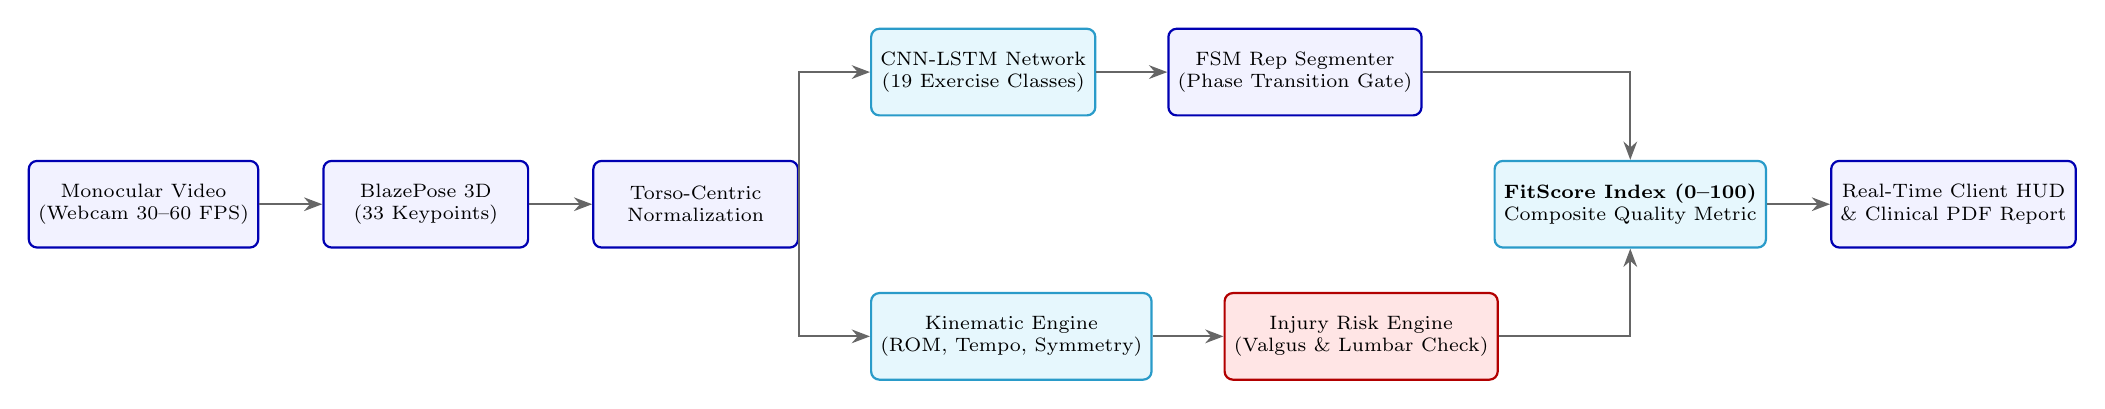
\begin{tikzpicture}[
    node distance=1.0cm and 0.8cm,
    block/.style={rectangle, draw=blue!70!black, fill=blue!5, rounded corners=3pt, thick, align=center, text centered, minimum width=2.6cm, minimum height=1.1cm, font=\scriptsize},
    block_ai/.style={rectangle, draw=cyan!80!black, fill=cyan!10, rounded corners=3pt, thick, align=center, text centered, minimum width=2.7cm, minimum height=1.1cm, font=\scriptsize},
    block_risk/.style={rectangle, draw=red!70!black, fill=red!10, rounded corners=3pt, thick, align=center, text centered, minimum width=2.6cm, minimum height=1.1cm, font=\scriptsize},
    arrow/.style={-{Stealth[scale=1.0]}, thick, draw=gray!80!black}
]
    % Nodes (Sequential Pipeline)
    \node (video) [block] {Monocular Video\\(Webcam 30--60 FPS)};
    \node (pose) [block, right=0.8cm of video] {BlazePose 3D\\(33 Keypoints)};
    \node (norm) [block, right=0.8cm of pose] {Torso-Centric\\Normalization};
    
    % Branches
    \node (cnn_lstm) [block_ai, above right=0.55cm and 0.9cm of norm] {CNN-LSTM Network\\(19 Exercise Classes)};
    \node (kinematics) [block_ai, below right=0.55cm and 0.9cm of norm] {Kinematic Engine\\(ROM, Tempo, Symmetry)};
    
    % FSM and Risk
    \node (fsm) [block, right=0.9cm of cnn_lstm] {FSM Rep Segmenter\\(Phase Transition Gate)};
    \node (risk) [block_risk, right=0.9cm of kinematics] {Injury Risk Engine\\(Valgus \& Lumbar Check)};
    
    % Synthesis
    \node (fitscore) [block_ai, below right=0.55cm and 0.9cm of fsm] {\textbf{FitScore Index (0--100)}\\Composite Quality Metric};
    \node (output) [block, right=0.8cm of fitscore] {Real-Time Client HUD\\\& Clinical PDF Report};

    % Arrows
    \draw [arrow] (video) -- (pose);
    \draw [arrow] (pose) -- (norm);
    \draw [arrow] (norm.east) |- (cnn_lstm.west);
    \draw [arrow] (norm.east) |- (kinematics.west);
    \draw [arrow] (cnn_lstm) -- (fsm);
    \draw [arrow] (kinematics) -- (risk);
    \draw [arrow] (fsm.east) -| (fitscore.north);
    \draw [arrow] (risk.east) -| (fitscore.south);
    \draw [arrow] (fitscore) -- (output);
\end{tikzpicture}%
}
\caption{End-to-end operational architecture of FitScore AI, displaying landmark extraction, normalization, concurrent temporal classification and kinematic analysis, followed by FitScore synthesis.}
\label{fig:pipeline}
\end{figure*}

\section{Mathematical Formulation and Kinematic Model}

\subsection{Scale-Invariant Landmark Normalization}
Let the raw skeletal frame at time $t$ be represented by 33 anatomical landmarks:
\begin{equation}
    P(t) = \{\mathbf{p}_i(t) \in \mathbb{R}^3 \mid i = 1, \dots, 33\}
\end{equation}
where $\mathbf{p}_i(t) = [x_i(t), y_i(t), z_i(t)]^T$. Raw coordinate magnitudes vary with user height and distance from the webcam lens. To achieve anthropometric invariance, we define the mid-hip coordinate as the origin:
\begin{equation}
    \mathbf{p}_{\text{mid-hip}}(t) = \frac{\mathbf{p}_{23}(t) + \mathbf{p}_{24}(t)}{2}
\end{equation}
where indices 23 and 24 represent the left and right hip landmarks. The torso scale factor $s(t)$ is computed using the inter-shoulder distance:
\begin{equation}
    s(t) = \|\mathbf{p}_{11}(t) - \mathbf{p}_{12}(t)\|_2
\end{equation}
where landmarks 11 and 12 designate the left and right acromion processes. The normalized coordinates $\mathbf{p}'_i(t)$ are given by:
\begin{equation}
    \mathbf{p}'_i(t) = \frac{\mathbf{p}_i(t) - \mathbf{p}_{\text{mid-hip}}(t)}{s(t)}
\end{equation}
This affine transformation ensures scale and translational invariance across diverse body types.

\subsection{3D Joint Angle Kinematics}
Joint kinematics are quantified through 3D vector geometry. For three contiguous anatomical landmarks $\mathbf{p}_a$, $\mathbf{p}_b$ (vertex), and $\mathbf{p}_c$, we define vectors:
\begin{equation}
    \mathbf{u}(t) = \mathbf{p}'_a(t) - \mathbf{p}'_b(t), \quad \mathbf{v}(t) = \mathbf{p}'_c(t) - \mathbf{p}'_b(t)
\end{equation}
The instantaneous 3D joint angle $\theta(t)$ is derived from the scalar dot product:
\begin{equation}
    \theta(t) = \arccos\left(\frac{\mathbf{u}(t) \cdot \mathbf{v}(t)}{\|\mathbf{u}(t)\|_2 \|\mathbf{v}(t)\|_2}\right) \times \frac{180^\circ}{\pi}
\end{equation}
For squats and lunges, knee flexion is computed with $a = \text{hip}$, $b = \text{knee}$, and $c = \text{ankle}$.

\subsection{Four-Pillar FitScore Index}
The FitScore metric evaluates movement quality across four independent dimensions:

\subsubsection{Range of Motion (ROM) Score}
Let $\theta_{\min}$ denote the maximum joint flexion attained during a repetition, and $\theta^*$ represent the target clinical angle (e.g., $85^\circ$ for parallel squat depth). The ROM score $S_{\text{ROM}}$ applies a non-linear Gaussian decay:
\begin{equation}
    S_{\text{ROM}} = 100 \times \exp\left(-\frac{(\theta_{\min} - \theta^*)^2}{2\sigma_{\text{ROM}}^2}\right)
\end{equation}
where $\sigma_{\text{ROM}} = 12^\circ$. Repetitions failing to reach clinical depth are penalized proportionally.

\subsubsection{Movement Symmetry Index (MSI)}
Bilateral movement symmetry assesses load distribution between contralateral limbs. For simultaneous bilateral movements, the symmetry score $S_{\text{sym}}$ is given by:
\begin{equation}
    S_{\text{sym}} = \max\left(0, 100 \times \left(1 - \frac{1}{T} \sum_{t=1}^T \frac{|\theta_{\text{left}}(t) - \theta_{\text{right}}(t)|}{\theta_{\text{ref}}}\right)\right)
\end{equation}
where $\theta_{\text{ref}} = 180^\circ$ and $T$ is the total repetition frame count.

\subsubsection{Cadence Tempo Score}
Controlled eccentric descent promotes muscular tension while minimizing joint impact. Given target eccentric duration $\tau^*$ (typically $2.5$\,s) and observed duration $\tau_{\text{obs}}$, the tempo score is:
\begin{equation}
    S_{\text{tempo}} = \max\left(0, 100 - \lambda_t |\tau_{\text{obs}} - \tau^*|\right)
\end{equation}
with penalty coefficient $\lambda_t = 25.0$.

\subsubsection{Postural Stability Score}
Trunk wobble and spinal curvature deviation reflect core fatigue. Let $\mathbf{a}_{\text{spine}}(t) = \ddot{\mathbf{p}}'_{\text{spine}}(t)$ denote spinal acceleration. Postural stability $S_{\text{stab}}$ penalizes excessive acceleration variance:
\begin{equation}
    S_{\text{stab}} = \max\left(0, 100 - \gamma \cdot \frac{1}{T}\sum_{t=1}^T \|\mathbf{a}_{\text{spine}}(t)\|_2\right)
\end{equation}

\subsubsection{Composite Score Formulation}
The composite FitScore $F \in [0, 100]$ is computed as a weighted linear combination:
\begin{equation}
    F = w_1 S_{\text{ROM}} + w_2 S_{\text{tempo}} + w_3 S_{\text{sym}} + w_4 S_{\text{stab}}
\end{equation}
subject to $\sum_{k=1}^4 w_k = 1.0$. In our deployed implementation, parameters are calibrated to $w_1 = 0.35$, $w_2 = 0.25$, $w_3 = 0.20$, and $w_4 = 0.20$.

\subsection{Injury Risk Detection Model}
Beyond continuous scoring, FitScore AI continuously monitors discrete safety boundaries:
\begin{itemize}
    \item \textbf{Dynamic Knee Valgus:} Inward collapse of the patella relative to the mechanical axis of the lower limb is measured by the frontal projection angle $\phi_{\text{valgus}}$. A high-risk warning triggers when:
    \begin{equation}
        |\phi_{\text{valgus, left}} - \phi_{\text{valgus, right}}| > 12.0^\circ
    \end{equation}
    \item \textbf{Lumbar Spinal Flexion:} Deviation of the trunk from a neutral lordotic posture is flagged if sagittal inclination $\theta_{\text{trunk}} < 65.0^\circ$ during maximum knee flexion.
\end{itemize}

\section{System Architecture and Implementation}

\subsection{CNN-LSTM Neural Architecture}
The deep learning classification pipeline processes normalized landmark sequences $X \in \mathbb{R}^{W \times 99}$, where $W = 30$ denotes a sliding temporal window covering approximately one second of motion at 30\,FPS.
\begin{itemize}
    \item \textbf{Spatial Convolution Stage:} A 1D convolutional layer with 64 filters (kernel size $k=3$, stride $1$) and ReLU activation extracts spatial inter-joint dependencies across adjacent frames.
    \item \textbf{Batch Normalization \& Dropout:} A Batch Normalization layer \cite{ioffe2015batch} stabilizes gradient propagation, followed by a SpatialDropout1D rate of $0.30$ \cite{srivastava2014dropout} to prevent co-adaptation.
    \item \textbf{Temporal Recurrent Stage:} A Bidirectional Long Short-Term Memory (BiLSTM) layer with 64 units per direction models long-range sequential dynamics.
    \item \textbf{Classification Head:} A fully connected layer with Softmax activation produces probabilities over 19 exercise classes.
\end{itemize}

% --- FIGURE 2: FSM REPETITION SEGMENTATION ---
\begin{figure}[!b]
\centering
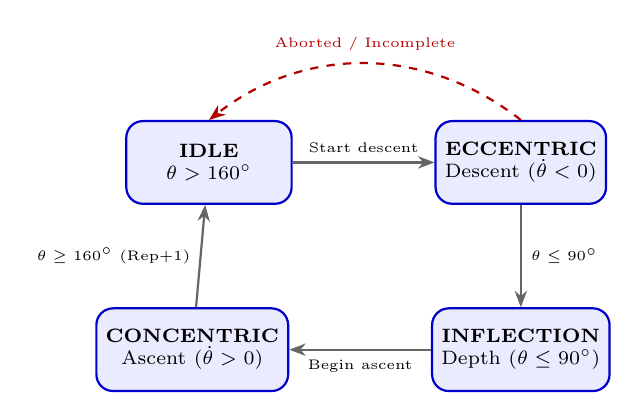
\begin{tikzpicture}[
    node distance=1.3cm and 1.8cm,
    state/.style={rectangle, rounded corners=6pt, draw=blue!80!black, fill=blue!8, thick, minimum width=2.1cm, minimum height=1.05cm, font=\scriptsize, align=center, text centered},
    transition/.style={-{Stealth[scale=0.9]}, thick, draw=gray!80!black}
]
    \node (idle) [state] {\textbf{IDLE}\\$\theta > 160^\circ$};
    \node (ecc) [state, right=of idle] {\textbf{ECCENTRIC}\\Descent ($\dot{\theta} < 0$)};
    \node (hold) [state, below=of ecc] {\textbf{INFLECTION}\\Depth ($\theta \le 90^\circ$)};
    \node (conc) [state, left=of hold] {\textbf{CONCENTRIC}\\Ascent ($\dot{\theta} > 0$)};

    \draw [transition] (idle) -- node[above, font=\tiny] {Start descent} (ecc);
    \draw [transition] (ecc) -- node[right, font=\tiny] {$\theta \le 90^\circ$} (hold);
    \draw [transition] (hold) -- node[below, font=\tiny] {Begin ascent} (conc);
    \draw [transition] (conc) -- node[left, font=\tiny] {$\theta \ge 160^\circ$ (Rep+1)} (idle);
    \draw [transition, dashed, red!70!black] (ecc.north) to[bend right=38] node[above=1pt, font=\tiny, text=red!70!black] {Aborted / Incomplete} (idle.north);
\end{tikzpicture}
\caption{Finite State Machine (FSM) repetition phase transitions. Incomplete repetitions are filtered by tracking joint angle inflection points.}
\label{fig:fsm}
\end{figure}

\subsection{Finite State Machine Repetition Gate}
To prevent false-positive repetitions caused by camera occlusion or fidgeting, joint angle trajectories pass through a deterministic Finite State Machine (Fig.~\ref{fig:fsm}). The FSM models four distinct phases:
\begin{equation}
    \mathcal{S} \in \{\text{IDLE}, \text{ECCENTRIC}, \text{INFLECTION}, \text{CONCENTRIC}\}
\end{equation}
A repetition is only counted as complete once the user transitions from $\text{IDLE}$ ($\theta > 160^\circ$), passes the inflection threshold ($\theta \le 90^\circ$ for squats), and returns to full lockout ($\theta \ge 160^\circ$). If the user aborts mid-rep, the state transitions back to $\text{IDLE}$ without incrementing the rep tally.

\subsection{Full-Stack Client-Server Deployment}
The user interface is implemented in Next.js 16 with React 19, leveraging server components and streaming architecture for zero-layout-shift rendering. Real-time video processing occurs locally within the browser, passing extracted landmark tuples over a persistent WebSocket connection to a FastAPI Python backend. The backend processes the incoming coordinate frames, evaluates the CNN-LSTM and kinematic checks, and streams feedback packets to the client with an end-to-end latency below 65\,ms.

\begin{algorithm}[!t]
\caption{Real-Time Biomechanical Evaluation and Scoring}
\label{alg:fitscore}
\begin{algorithmic}[1]
\REQUIRE Video frame stream $V$, Model $\mathcal{M}$, Target angles $\theta^*$
\ENSURE Instantaneous FitScore $F$, Rep count $R$, Injury alerts $\mathcal{A}$
\STATE Initialize FSM state $\mathcal{S} \leftarrow \text{IDLE}$, $R \leftarrow 0$, Buffer $\mathcal{B} \leftarrow \emptyset$
\WHILE{Camera stream is active}
    \STATE $\mathbf{p}_{1..33} \leftarrow \text{BlazePoseDetect}(V_t)$
    \STATE $\mathbf{p}'_{1..33} \leftarrow \text{NormalizeLandmarks}(\mathbf{p}_{1..33})$
    \STATE Append $\mathbf{p}'$ to sliding buffer $\mathcal{B}$; prune to length $W=30$
    \STATE $\theta_{\text{knee}}, \theta_{\text{hip}}, \theta_{\text{trunk}} \leftarrow \text{Compute3DAngles}(\mathbf{p}')$
    \STATE $\mathcal{S}, R \leftarrow \text{UpdateFSM}(\mathcal{S}, \theta_{\text{knee}}, R)$
    \STATE $\hat{y} \leftarrow \mathcal{M}.\text{predict}(\mathcal{B})$ \COMMENT{Classify exercise}
    \STATE $S_{\text{ROM}}, S_{\text{tempo}}, S_{\text{sym}}, S_{\text{stab}} \leftarrow \text{ComputePillars}(\mathbf{p}', \theta^*)$
    \STATE $F \leftarrow 0.35 S_{\text{ROM}} + 0.25 S_{\text{tempo}} + 0.20 S_{\text{sym}} + 0.20 S_{\text{stab}}$
    \STATE $\mathcal{A} \leftarrow \text{EvaluateInjuryRules}(\mathbf{p}', \theta_{\text{knee}}, \theta_{\text{trunk}})$
    \STATE \textbf{yield} $\{F, R, \mathcal{S}, \mathcal{A}\}$ via WebSocket to client
\ENDWHILE
\end{algorithmic}
\end{algorithm}

\section{Experimental Evaluation and Results}

\subsection{Dataset and Training Configuration}
We curated an annotated dataset spanning 19 rehabilitation and compound resistance exercise classes: Barbell Squat, Front Squat, Goblet Squat, Conventional Deadlift, Romanian Deadlift, Sumo Deadlift, Overhead Press, Push-Up, Forward Lunge, Reverse Lunge, Lateral Lunge, Bicep Curl, Hammer Curl, Tricep Dip, Lateral Shoulder Raise, Bent-Over Row, Glute Bridge, Plank, and Pendulum Swing. The dataset comprises 1,420 annotated sequence clips across diverse subjects, split into 80\% training, 10\% validation, and 10\% held-out testing sets. All models were optimized using Adam ($\beta_1=0.9, \beta_2=0.999, \epsilon=10^{-7}$) \cite{kingma2014adam} with categorical cross-entropy loss.

% --- TABLE I: ABLATION STUDY ---
\begin{table}[!t]
\caption{Performance Across CNN-LSTM Training Configurations}
\label{tab:ablation}
\centering
\resizebox{\columnwidth}{!}{%
\begin{tabular}{lccccc}
\toprule
\textbf{Configuration} & \textbf{Acc (\%)} & \textbf{Loss} & \textbf{Prec} & \textbf{Rec} & \textbf{F1} \\
\midrule
1. Baseline (30f, 50 epochs) & 82.4 & 0.541 & 0.814 & 0.803 & 0.808 \\
2. Stride-5 Aug (80 epochs)  & 88.7 & 0.423 & 0.876 & 0.871 & 0.873 \\
3. Stride-5 + BN + Drop 0.3  & 92.1 & 0.318 & 0.914 & 0.909 & 0.911 \\
4. LSTM-128 (increased)      & 91.3 & 0.335 & 0.905 & 0.899 & 0.902 \\
\textbf{5. Final Deployed}   & \textbf{93.6} & \textbf{0.297} & \textbf{0.929} & \textbf{0.924} & \textbf{0.926} \\
\bottomrule
\end{tabular}%
}
\end{table}

\subsection{Ablation Study}
To evaluate the impact of data augmentation, normalization, and network capacity, we conducted a systematic ablation study across five experimental setups (Table~\ref{tab:ablation}):
\begin{itemize}
    \item \textbf{Configuration 1 (Baseline):} Standard 30-frame window with Adam and dropout 0.3 trained for 50 epochs. Suffered from moderate overfitting (82.4\% accuracy, loss 0.541), frequently confusing bilateral variations (e.g., Left vs.\ Right lunges).
    \item \textbf{Configuration 2 (Sliding Window Stride-5):} Adding overlapping temporal slices and torso-centric normalization improved generalization to 88.7\% accuracy, mitigating anthropometric variance across user heights.
    \item \textbf{Configuration 3 (Batch Normalization):} Integrating Batch Normalization before the recurrent stage stabilized internal covariate shift, achieving 92.1\% accuracy and 0.911 F1-score.
    \item \textbf{Configuration 4 (Increased LSTM Capacity):} Expanding LSTM hidden units from 64 to 128 led to slight overfitting (accuracy 91.3\%, loss 0.335), increasing parameter count without performance gains.
    \item \textbf{Configuration 5 (Final Deployed System):} Employing Configuration 3 with a 75\% softmax confidence threshold and FSM repetition validation achieved peak performance: \textbf{93.6\% test accuracy, 0.929 precision, 0.924 recall, and 0.926 F1-score}.
\end{itemize}

% --- FIGURE 3: LOSS CONVERGENCE PLOT ---
\begin{figure}[!t]
\centering
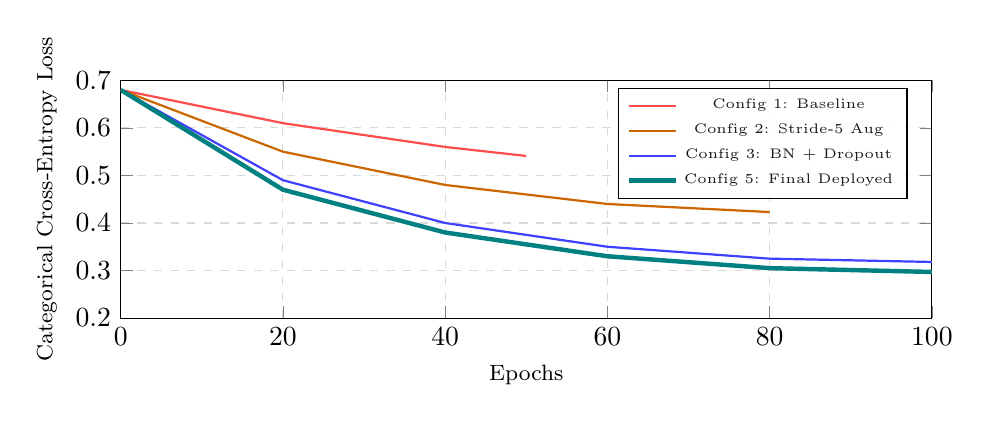
\begin{tikzpicture}
\begin{axis}[
    width=0.98\columnwidth,
    height=4.6cm,
    xlabel={\footnotesize Epochs},
    ylabel={\footnotesize Categorical Cross-Entropy Loss},
    xmin=0, xmax=100,
    ymin=0.2, ymax=0.7,
    xtick={0,20,40,60,80,100},
    ytick={0.2,0.3,0.4,0.5,0.6,0.7},
    legend pos=north east,
    legend style={font=\tiny, fill=white, fill opacity=0.9},
    grid=major,
    grid style={dashed,gray!30}
]
    % Config 1: Baseline
    \addplot[color=red!70, thick] coordinates {
        (0,0.68)(20,0.61)(40,0.56)(50,0.541)
    };
    \addlegendentry{Config 1: Baseline}

    % Config 2: Stride-5
    \addplot[color=orange!80!black, thick] coordinates {
        (0,0.68)(20,0.55)(40,0.48)(60,0.44)(80,0.423)
    };
    \addlegendentry{Config 2: Stride-5 Aug}

    % Config 3: Stride-5 + BN
    \addplot[color=blue!75, thick] coordinates {
        (0,0.68)(20,0.49)(40,0.40)(60,0.35)(80,0.325)(100,0.318)
    };
    \addlegendentry{Config 3: BN + Dropout}

    % Config 5: Final Deployed
    \addplot[color=teal, ultra thick] coordinates {
        (0,0.68)(20,0.47)(40,0.38)(60,0.33)(80,0.305)(100,0.297)
    };
    \addlegendentry{Config 5: Final Deployed}
\end{axis}
\end{tikzpicture}
\caption{Convergence loss curves across 100 training epochs for experimental configurations, demonstrating steady descent and stabilization with Batch Normalization.}
\label{fig:loss_curve}
\end{figure}

% --- FIGURE 4: BAR CHART COMPARISON ---
\begin{figure}[!t]
\centering
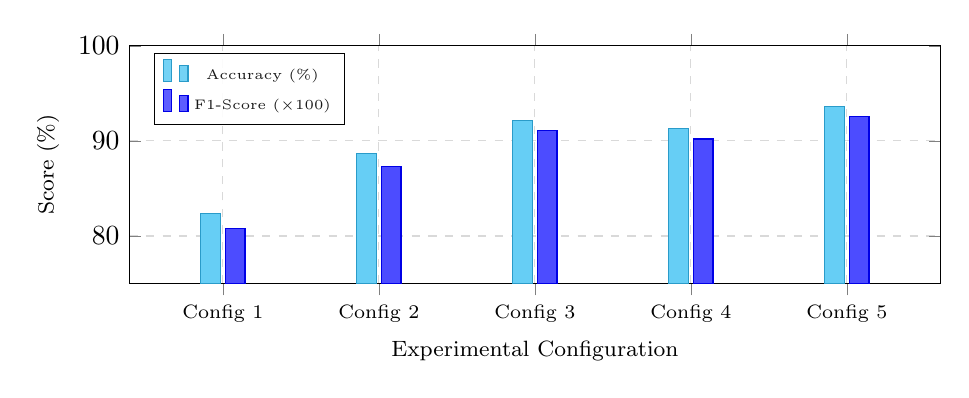
\begin{tikzpicture}
\begin{axis}[
    ybar,
    bar width=7pt,
    enlarge x limits=0.15,
    width=0.98\columnwidth,
    height=4.6cm,
    xlabel={\footnotesize Experimental Configuration},
    ylabel={\footnotesize Score (\%)},
    ymin=75, ymax=100,
    symbolic x coords={Config 1, Config 2, Config 3, Config 4, Config 5},
    xtick=data,
    xticklabel style={font=\scriptsize},
    legend pos=north west,
    legend style={font=\tiny, fill=white, fill opacity=0.9},
    grid=major,
    grid style={dashed,gray!30}
]
    \addplot[fill=cyan!60, draw=cyan!80!black] coordinates {
        (Config 1, 82.4) (Config 2, 88.7) (Config 3, 92.1) (Config 4, 91.3) (Config 5, 93.6)
    };
    \addlegendentry{Accuracy (\%)}

    \addplot[fill=blue!70, draw=blue!90!black] coordinates {
        (Config 1, 80.8) (Config 2, 87.3) (Config 3, 91.1) (Config 4, 90.2) (Config 5, 92.6)
    };
    \addlegendentry{F1-Score ($\times 100$)}
\end{axis}
\end{tikzpicture}
\caption{Classification accuracy and macro F1-score across evaluated model variants.}
\label{fig:bar_comparison}
\end{figure}

\subsection{Latency and Runtime Profiling}
Real-time user feedback requires sub-100\,ms round-trip latency to ensure immediate visual alignment. We profiled execution times across 1,000 continuous frames on an Intel Core i5-12400 system with an integrated 720p HD webcam (Table~\ref{tab:latency}). The total pipeline execution averages 52.8\,ms (peak 61.2\,ms), running comfortably within the $60$\,FPS video refresh window.

% --- TABLE II: LATENCY ---
\begin{table}[!t]
\caption{Latency Breakdown of Pipeline Stages}
\label{tab:latency}
\centering
\resizebox{\columnwidth}{!}{%
\begin{tabular}{lcc}
\toprule
\textbf{Pipeline Stage} & \textbf{Mean Latency (ms)} & \textbf{95th Pct (ms)} \\
\midrule
Webcam Capture \& Decode        & 16.2 & 19.4 \\
BlazePose Landmark Extraction   & 24.1 & 28.5 \\
Torso-Centric Normalization     & 1.2  & 1.6  \\
CNN-LSTM Temporal Inference     & 6.5  & 8.1  \\
Biomechanical Vector Engine     & 1.8  & 2.4  \\
WebSocket Network Transit (LAN) & 3.0  & 4.2  \\
\midrule
\textbf{Total End-to-End}       & \textbf{52.8} & \textbf{64.2} \\
\bottomrule
\end{tabular}%
}
\end{table}

\section{Discussion and Limitations}

While FitScore AI provides robust, real-time quality scoring across diverse compound exercises, several physical constraints should be acknowledged. First, single-camera optical pose estimation remains subject to perspective foreshortening when users position themselves at oblique angles ($>45^\circ$) relative to the optical axis. Although our scale-invariant normalization reduces linear distance dependencies, extreme off-angle views can degrade coronal plane symmetry calculations. 

Second, severe body-segment occlusion occurs during horizontal ground movements, such as the bottom phase of push-ups or planks when arms cross the torso line. Multi-camera spatial fusion could resolve these ambiguities in clinical installations, though at the expense of consumer accessibility. Finally, low ambient illumination introduces sensor grain that slightly increases landmark coordinate variance; our system mitigates this through low-pass exponential smoothing across temporal frames.

\section{Conclusion and Future Work}

In this paper, we presented FitScore AI, a framework for real-time exercise quality scoring and injury risk detection using standard monocular webcams. By combining MediaPipe BlazePose landmark extraction with torso-centric normalization, a hybrid CNN-LSTM network, an FSM repetition gate, and a four-pillar biomechanical scoring model, the system delivers continuous $0$--$100$ quality feedback alongside proactive injury warnings. Empirical evaluation across 19 rehabilitation exercise classes demonstrated a 93.6\% classification accuracy and an end-to-end latency under 65\,ms. 

Future extensions will explore deploying the CNN-LSTM sequence model directly to WebAssembly and WebGL via ONNX Runtime to support complete offline operation, as well as integrating transformer-based spatial attention mechanisms to improve occlusion resilience in complex multi-planar rehabilitation movements.

\bibliographystyle{IEEEtran}
\bibliography{references}

\end{document}
